PHATE (Potential of Heat-diffusion for Affinity-based Trajectory Embedding) is an unsupervised method for dimensionality reduction and visualization of biological data \cite{moon2019visualizing}. A preprint of the paper introducing PHATE \citep{moon2017phate} states that the method was inspired by word-embedding techniques such as Word2vec. Despite its roots in word embeddings, PHATE has not yet been applied to textual data. In this paper, we demonstrate that PHATE generalizes well to natural language data \footnote{Code and data available here: \url{https://anonymous.4open.science/r/phate-for-text-4D7D/README.md}.}, producing meaningful embeddings whose trajectories encode "narrative arcs."

\begin{figure}
    \centering
    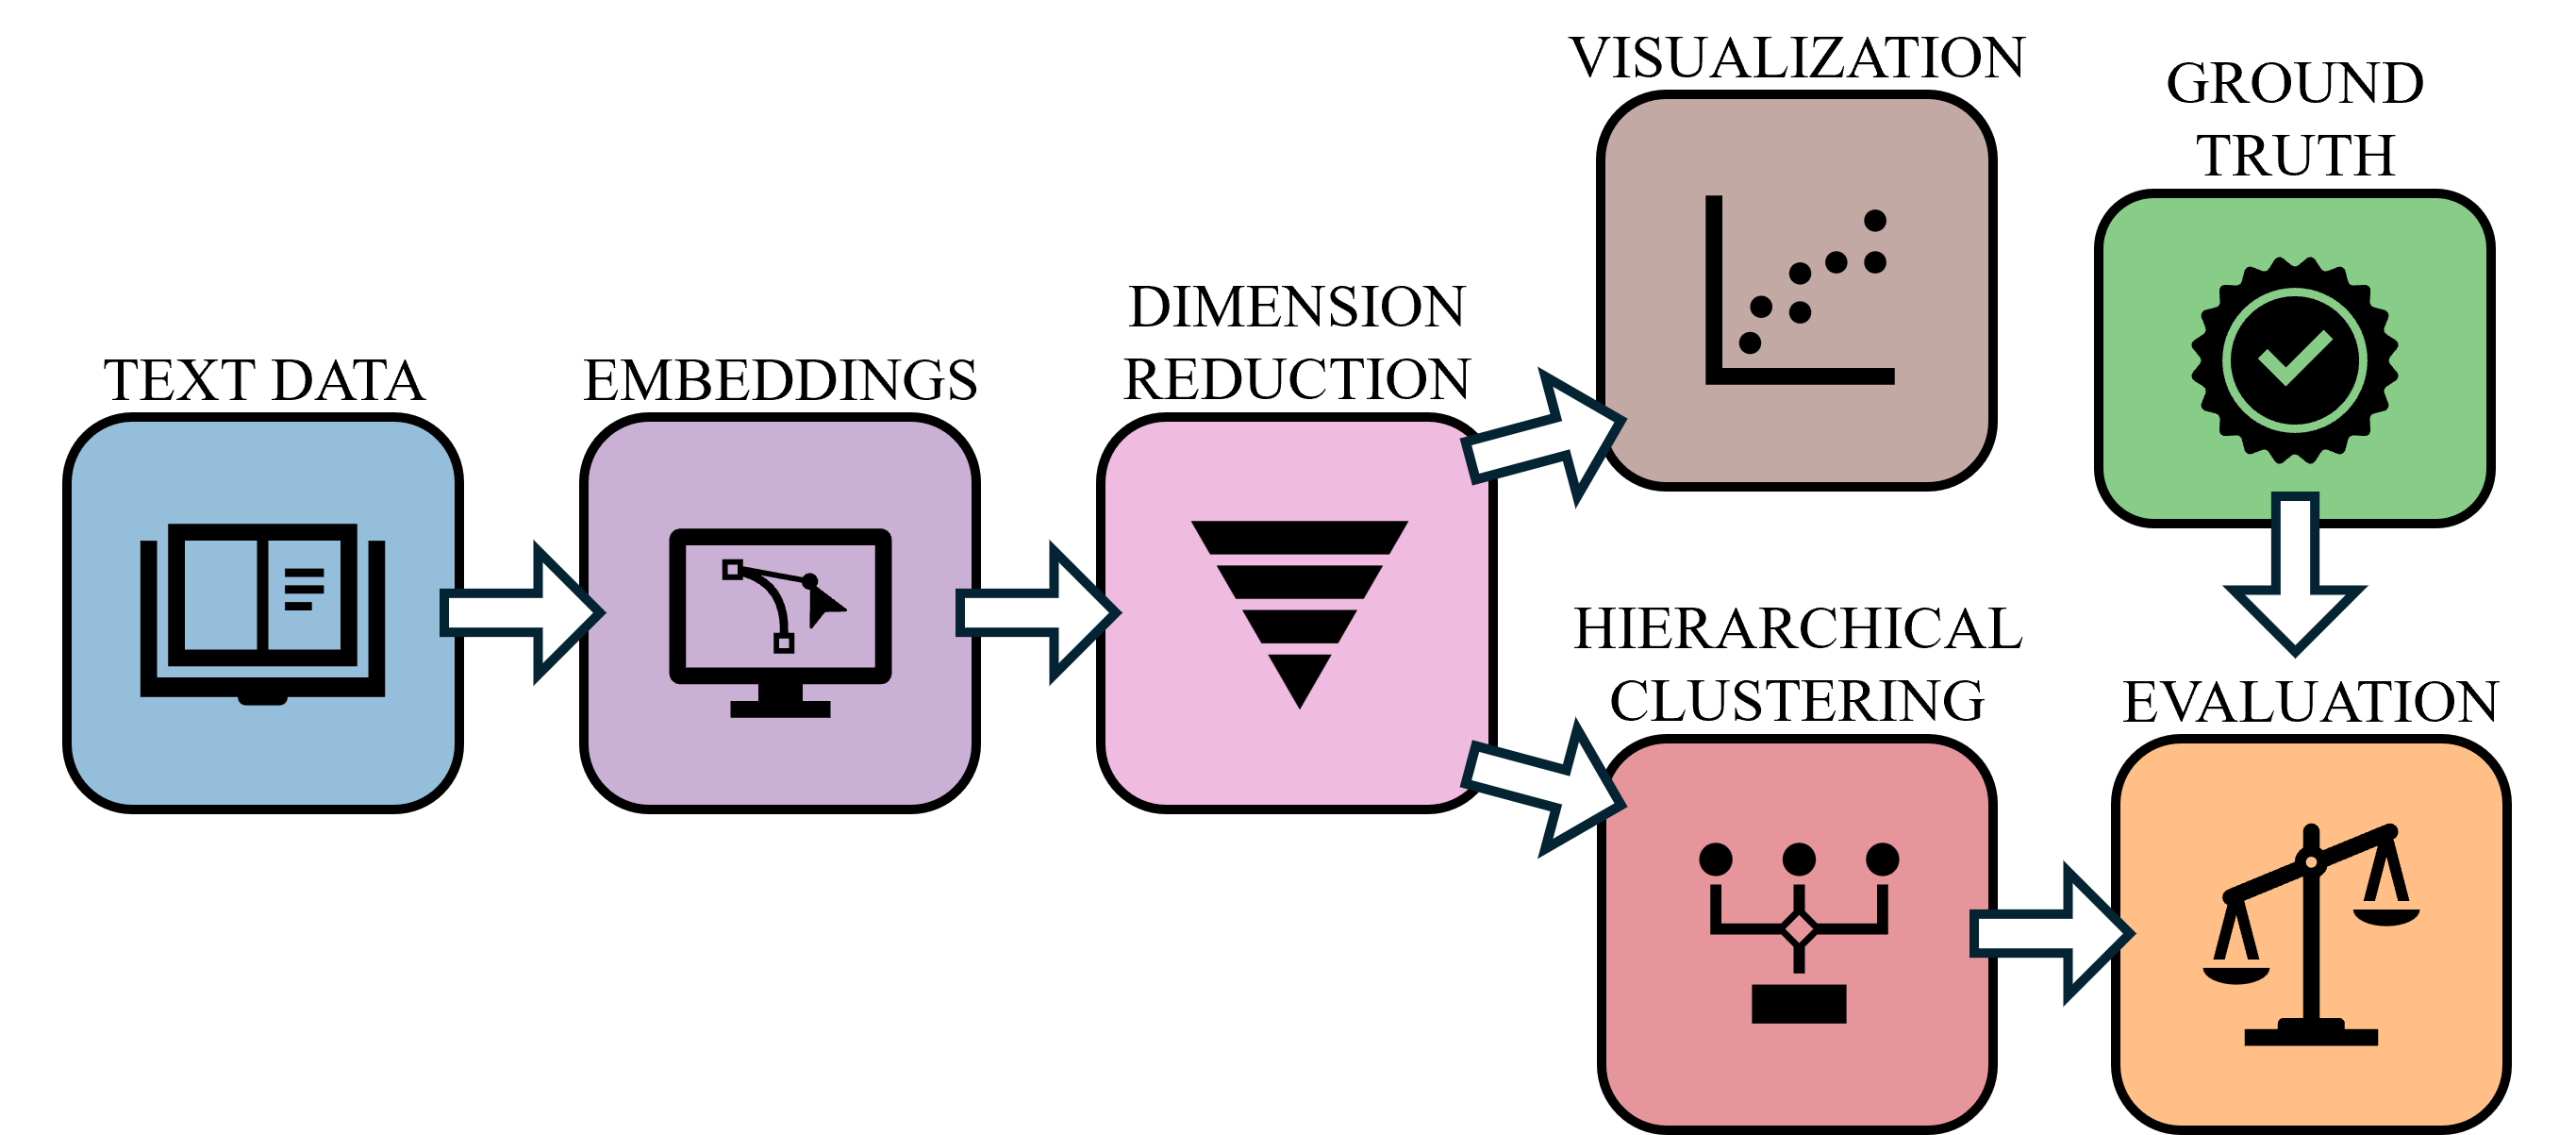
\includegraphics[width=1\linewidth]{workflow.png}
    \caption{The workflow used for studying PHATE for visualization and hierarchical clustering of text}
    \label{fig:workflow}
\end{figure}

We show that a multiscale variant of PHATE \cite{kuchroo2022multiscale} is competitive with popular hierarchical clustering pipelines that combine UMAP or PCA with agglomerative clustering or HDBSCAN. We further apply this method to a newly curated dataset of environmental policy narratives from US stakeholders, finding that PHATE yields more informative visualizations than standard approaches. These results open the door to new modes of textual analysis and motivate further extensions of PHATE beyond biological domains.